\documentclass[30pt,twocolumn,letterpaper]{article}
\usepackage{cvpr}
\usepackage{times}
\usepackage{booktabs}
\usepackage{epsfig}
\usepackage{graphicx}
\usepackage{amsmath}
\usepackage{amssymb}
\cvprfinalcopy
\def\cvprPaperID{****}
\def\httilde{\mbox{\tt\raisebox{-.5ex}{\symbol{126}}}}
\usepackage{graphicx}
\usepackage{indentfirst}
\setlength{\parindent}{2em}
\usepackage{cite}
\usepackage[colorlinks,linkcolor=red,anchorcolor=blue,citecolor=green,backref=page]{hyperref}
\author{Qilei Zhang}
\date{May 29 2018}
\title{Optical systems}
\begin{document}
\maketitle
\begin{abstract}
   The development of stochastic resonance took a large leap forward when its potential relevance for neurophysiological processes had been recognized. Longtin, Bulsara, and Moss  observed that interspike interval histograms of periodically stimulated neurons exhibit a remarkable resemblance to residence-time distributions of periodically driven bistable systems.
\end{abstract}
\section{Introduction}
In this section, we report on the relevant neurophysiological experiments and describe how stochastic resonance enters naturally into standard models for neuronal dynamics. By now, stochastic resonance is a well accepted paradigm in the biological and neurophysiological sciences, and several recent reviews on neurophysiological applications of stochastic resonance are available\cite{Benzi1983A}.
\begin{figure}[htbp]
\small
\centering
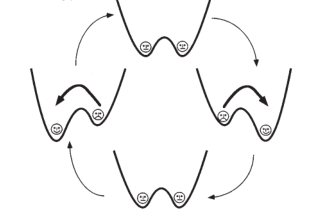
\includegraphics[width=20em]{000.png}
\caption{23 Bistable ring laser}
\label{fig:lable}
\end{figure}
\section{Neurophysiological background}
There is a large variety of types of neurons in the nervous system of animals and humans with variations in structure, function, and size. Let us restrict ourselves here to a canonical neuron, which presents the underlying functional skeleton for all neurons. The canonical neuron is divided into three parts, an input part, a processing part, and a signal transmission part\cite{Gammaitoni1995Stochastic}. \\
\begin{equation}
\quad x'=x-x^3+u(t)+A_0 cos(st)
\end{equation}
\begin{table}
\begin{center}
\begin{tabular}{cccccccc}
\toprule
         & 1 &  2  &   3  &  4  &  5  &  6  & 7 \\
\midrule
Alphabet & A &  B  &   C  &  D  &  E  &  F  & G\\
Roman    & I &  II &  III &  IV &  V  &  VI & VII\\
\bottomrule
\end{tabular}
\end{center}
\caption{Results.   Ours is better.}
\end{table}
\section{Neuron firing and Poissonian spike trains}
Wiesenfeld, Pierson, Pantazelou, Dames, and Moss proposed a very elegant approximate theory for modeling neuron firing in the presence of noise and a periodic stimulus. The neuron emits uncorrelated, sharp spikes at random times t n . The spiking rate, however, is inhomogeneous, i.e., sinusoidally modulated. This sort of process is described by the theory of inhomogeneous Poissonian point processes��see\cite{Hu1990Periodically}.
{\small
\bibliographystyle{ieee}
\bibliography{1}
}
\end{document}
